% Graphic for TeX using PGF
% Title: D:\jpaper\UML.dia
% Creator: Dia v0.97.2
% CreationDate: Wed May 13 11:28:56 2015
% For: amal029
% \usepackage{tikz}
% The following commands are not supported in PSTricks at present
% We define them conditionally, so when they are implemented,
% this pgf file will use them.
\ifx\du\undefined
  \newlength{\du}
\fi
\setlength{\du}{15\unitlength}
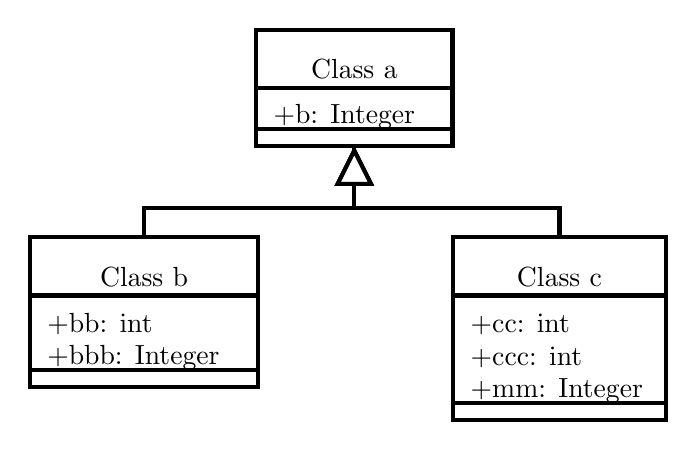
\begin{tikzpicture}
\pgftransformxscale{1.000000}
\pgftransformyscale{-1.000000}
\definecolor{dialinecolor}{rgb}{0.000000, 0.000000, 0.000000}
\pgfsetstrokecolor{dialinecolor}
\definecolor{dialinecolor}{rgb}{1.000000, 1.000000, 1.000000}
\pgfsetfillcolor{dialinecolor}
\pgfsetlinewidth{0.100000\du}
\pgfsetdash{}{0pt}
\definecolor{dialinecolor}{rgb}{1.000000, 1.000000, 1.000000}
\pgfsetfillcolor{dialinecolor}
\fill (20.500000\du,13.050000\du)--(20.500000\du,14.450000\du)--(26.005000\du,14.450000\du)--(26.005000\du,13.050000\du)--cycle;
\definecolor{dialinecolor}{rgb}{0.000000, 0.000000, 0.000000}
\pgfsetstrokecolor{dialinecolor}
\draw (20.500000\du,13.050000\du)--(20.500000\du,14.450000\du)--(26.005000\du,14.450000\du)--(26.005000\du,13.050000\du)--cycle;
% setfont left to latex
\definecolor{dialinecolor}{rgb}{0.000000, 0.000000, 0.000000}
\pgfsetstrokecolor{dialinecolor}
\node at (23.252500\du,14.000000\du){Class b};
\definecolor{dialinecolor}{rgb}{1.000000, 1.000000, 1.000000}
\pgfsetfillcolor{dialinecolor}
\fill (20.500000\du,14.450000\du)--(20.500000\du,16.250000\du)--(26.005000\du,16.250000\du)--(26.005000\du,14.450000\du)--cycle;
\definecolor{dialinecolor}{rgb}{0.000000, 0.000000, 0.000000}
\pgfsetstrokecolor{dialinecolor}
\draw (20.500000\du,14.450000\du)--(20.500000\du,16.250000\du)--(26.005000\du,16.250000\du)--(26.005000\du,14.450000\du)--cycle;
% setfont left to latex
\definecolor{dialinecolor}{rgb}{0.000000, 0.000000, 0.000000}
\pgfsetstrokecolor{dialinecolor}
\node[anchor=west] at (20.650000\du,15.150000\du){+bb: int};
% setfont left to latex
\definecolor{dialinecolor}{rgb}{0.000000, 0.000000, 0.000000}
\pgfsetstrokecolor{dialinecolor}
\node[anchor=west] at (20.650000\du,15.950000\du){+bbb: Integer};
\definecolor{dialinecolor}{rgb}{1.000000, 1.000000, 1.000000}
\pgfsetfillcolor{dialinecolor}
\fill (20.500000\du,16.250000\du)--(20.500000\du,16.650000\du)--(26.005000\du,16.650000\du)--(26.005000\du,16.250000\du)--cycle;
\definecolor{dialinecolor}{rgb}{0.000000, 0.000000, 0.000000}
\pgfsetstrokecolor{dialinecolor}
\draw (20.500000\du,16.250000\du)--(20.500000\du,16.650000\du)--(26.005000\du,16.650000\du)--(26.005000\du,16.250000\du)--cycle;
\pgfsetlinewidth{0.100000\du}
\pgfsetdash{}{0pt}
\definecolor{dialinecolor}{rgb}{1.000000, 1.000000, 1.000000}
\pgfsetfillcolor{dialinecolor}
\fill (25.950000\du,8.050000\du)--(25.950000\du,9.450000\du)--(30.685000\du,9.450000\du)--(30.685000\du,8.050000\du)--cycle;
\definecolor{dialinecolor}{rgb}{0.000000, 0.000000, 0.000000}
\pgfsetstrokecolor{dialinecolor}
\draw (25.950000\du,8.050000\du)--(25.950000\du,9.450000\du)--(30.685000\du,9.450000\du)--(30.685000\du,8.050000\du)--cycle;
% setfont left to latex
\definecolor{dialinecolor}{rgb}{0.000000, 0.000000, 0.000000}
\pgfsetstrokecolor{dialinecolor}
\node at (28.317500\du,9.000000\du){Class a};
\definecolor{dialinecolor}{rgb}{1.000000, 1.000000, 1.000000}
\pgfsetfillcolor{dialinecolor}
\fill (25.950000\du,9.450000\du)--(25.950000\du,10.450000\du)--(30.685000\du,10.450000\du)--(30.685000\du,9.450000\du)--cycle;
\definecolor{dialinecolor}{rgb}{0.000000, 0.000000, 0.000000}
\pgfsetstrokecolor{dialinecolor}
\draw (25.950000\du,9.450000\du)--(25.950000\du,10.450000\du)--(30.685000\du,10.450000\du)--(30.685000\du,9.450000\du)--cycle;
% setfont left to latex
\definecolor{dialinecolor}{rgb}{0.000000, 0.000000, 0.000000}
\pgfsetstrokecolor{dialinecolor}
\node[anchor=west] at (26.100000\du,10.150000\du){+b: Integer};
\definecolor{dialinecolor}{rgb}{1.000000, 1.000000, 1.000000}
\pgfsetfillcolor{dialinecolor}
\fill (25.950000\du,10.450000\du)--(25.950000\du,10.850000\du)--(30.685000\du,10.850000\du)--(30.685000\du,10.450000\du)--cycle;
\definecolor{dialinecolor}{rgb}{0.000000, 0.000000, 0.000000}
\pgfsetstrokecolor{dialinecolor}
\draw (25.950000\du,10.450000\du)--(25.950000\du,10.850000\du)--(30.685000\du,10.850000\du)--(30.685000\du,10.450000\du)--cycle;
\pgfsetlinewidth{0.100000\du}
\pgfsetdash{}{0pt}
\definecolor{dialinecolor}{rgb}{1.000000, 1.000000, 1.000000}
\pgfsetfillcolor{dialinecolor}
\fill (30.700000\du,13.050000\du)--(30.700000\du,14.450000\du)--(35.820000\du,14.450000\du)--(35.820000\du,13.050000\du)--cycle;
\definecolor{dialinecolor}{rgb}{0.000000, 0.000000, 0.000000}
\pgfsetstrokecolor{dialinecolor}
\draw (30.700000\du,13.050000\du)--(30.700000\du,14.450000\du)--(35.820000\du,14.450000\du)--(35.820000\du,13.050000\du)--cycle;
% setfont left to latex
\definecolor{dialinecolor}{rgb}{0.000000, 0.000000, 0.000000}
\pgfsetstrokecolor{dialinecolor}
\node at (33.260000\du,14.000000\du){Class c};
\definecolor{dialinecolor}{rgb}{1.000000, 1.000000, 1.000000}
\pgfsetfillcolor{dialinecolor}
\fill (30.700000\du,14.450000\du)--(30.700000\du,17.050000\du)--(35.820000\du,17.050000\du)--(35.820000\du,14.450000\du)--cycle;
\definecolor{dialinecolor}{rgb}{0.000000, 0.000000, 0.000000}
\pgfsetstrokecolor{dialinecolor}
\draw (30.700000\du,14.450000\du)--(30.700000\du,17.050000\du)--(35.820000\du,17.050000\du)--(35.820000\du,14.450000\du)--cycle;
% setfont left to latex
\definecolor{dialinecolor}{rgb}{0.000000, 0.000000, 0.000000}
\pgfsetstrokecolor{dialinecolor}
\node[anchor=west] at (30.850000\du,15.150000\du){+cc: int};
% setfont left to latex
\definecolor{dialinecolor}{rgb}{0.000000, 0.000000, 0.000000}
\pgfsetstrokecolor{dialinecolor}
\node[anchor=west] at (30.850000\du,15.950000\du){+ccc: int};
% setfont left to latex
\definecolor{dialinecolor}{rgb}{0.000000, 0.000000, 0.000000}
\pgfsetstrokecolor{dialinecolor}
\node[anchor=west] at (30.850000\du,16.750000\du){+mm: Integer};
\definecolor{dialinecolor}{rgb}{1.000000, 1.000000, 1.000000}
\pgfsetfillcolor{dialinecolor}
\fill (30.700000\du,17.050000\du)--(30.700000\du,17.450000\du)--(35.820000\du,17.450000\du)--(35.820000\du,17.050000\du)--cycle;
\definecolor{dialinecolor}{rgb}{0.000000, 0.000000, 0.000000}
\pgfsetstrokecolor{dialinecolor}
\draw (30.700000\du,17.050000\du)--(30.700000\du,17.450000\du)--(35.820000\du,17.450000\du)--(35.820000\du,17.050000\du)--cycle;
\pgfsetlinewidth{0.100000\du}
\pgfsetdash{}{0pt}
\pgfsetmiterjoin
\pgfsetbuttcap
{
\definecolor{dialinecolor}{rgb}{0.000000, 0.000000, 0.000000}
\pgfsetfillcolor{dialinecolor}
% was here!!!
\definecolor{dialinecolor}{rgb}{0.000000, 0.000000, 0.000000}
\pgfsetstrokecolor{dialinecolor}
\draw (28.317500\du,10.850000\du)--(28.317500\du,12.350000\du)--(23.252500\du,12.350000\du)--(23.252500\du,13.050000\du);
}
\definecolor{dialinecolor}{rgb}{0.000000, 0.000000, 0.000000}
\pgfsetstrokecolor{dialinecolor}
\draw (28.317500\du,11.761803\du)--(28.317500\du,12.350000\du)--(23.252500\du,12.350000\du)--(23.252500\du,13.050000\du);
\pgfsetmiterjoin
\definecolor{dialinecolor}{rgb}{1.000000, 1.000000, 1.000000}
\pgfsetfillcolor{dialinecolor}
\fill (28.717500\du,11.761803\du)--(28.317500\du,10.961803\du)--(27.917500\du,11.761803\du)--cycle;
\pgfsetlinewidth{0.100000\du}
\pgfsetdash{}{0pt}
\pgfsetmiterjoin
\definecolor{dialinecolor}{rgb}{0.000000, 0.000000, 0.000000}
\pgfsetstrokecolor{dialinecolor}
\draw (28.717500\du,11.761803\du)--(28.317500\du,10.961803\du)--(27.917500\du,11.761803\du)--cycle;
% setfont left to latex
\pgfsetlinewidth{0.100000\du}
\pgfsetdash{}{0pt}
\pgfsetmiterjoin
\pgfsetbuttcap
{
\definecolor{dialinecolor}{rgb}{0.000000, 0.000000, 0.000000}
\pgfsetfillcolor{dialinecolor}
% was here!!!
\definecolor{dialinecolor}{rgb}{0.000000, 0.000000, 0.000000}
\pgfsetstrokecolor{dialinecolor}
\draw (28.317500\du,10.850000\du)--(28.317500\du,12.350000\du)--(33.260000\du,12.350000\du)--(33.260000\du,13.050000\du);
}
\definecolor{dialinecolor}{rgb}{0.000000, 0.000000, 0.000000}
\pgfsetstrokecolor{dialinecolor}
\draw (28.317500\du,11.761803\du)--(28.317500\du,12.350000\du)--(33.260000\du,12.350000\du)--(33.260000\du,13.050000\du);
\pgfsetmiterjoin
\definecolor{dialinecolor}{rgb}{1.000000, 1.000000, 1.000000}
\pgfsetfillcolor{dialinecolor}
\fill (28.717500\du,11.761803\du)--(28.317500\du,10.961803\du)--(27.917500\du,11.761803\du)--cycle;
\pgfsetlinewidth{0.100000\du}
\pgfsetdash{}{0pt}
\pgfsetmiterjoin
\definecolor{dialinecolor}{rgb}{0.000000, 0.000000, 0.000000}
\pgfsetstrokecolor{dialinecolor}
\draw (28.717500\du,11.761803\du)--(28.317500\du,10.961803\du)--(27.917500\du,11.761803\du)--cycle;
% setfont left to latex
\end{tikzpicture}
